\documentclass[]{article}
\usepackage{lmodern}
\usepackage{amssymb,amsmath}
\usepackage{ifxetex,ifluatex}
\usepackage{fixltx2e} % provides \textsubscript
\ifnum 0\ifxetex 1\fi\ifluatex 1\fi=0 % if pdftex
  \usepackage[T1]{fontenc}
  \usepackage[utf8]{inputenc}
\else % if luatex or xelatex
  \ifxetex
    \usepackage{mathspec}
    \usepackage{xltxtra,xunicode}
  \else
    \usepackage{fontspec}
  \fi
  \defaultfontfeatures{Mapping=tex-text,Scale=MatchLowercase}
  \newcommand{\euro}{€}
\fi
% use upquote if available, for straight quotes in verbatim environments
\IfFileExists{upquote.sty}{\usepackage{upquote}}{}
% use microtype if available
\IfFileExists{microtype.sty}{%
\usepackage{microtype}
\UseMicrotypeSet[protrusion]{basicmath} % disable protrusion for tt fonts
}{}
\usepackage[margin=1in]{geometry}
\usepackage{color}
\usepackage{fancyvrb}
\newcommand{\VerbBar}{|}
\newcommand{\VERB}{\Verb[commandchars=\\\{\}]}
\DefineVerbatimEnvironment{Highlighting}{Verbatim}{commandchars=\\\{\}}
% Add ',fontsize=\small' for more characters per line
\usepackage{framed}
\definecolor{shadecolor}{RGB}{248,248,248}
\newenvironment{Shaded}{\begin{snugshade}}{\end{snugshade}}
\newcommand{\KeywordTok}[1]{\textcolor[rgb]{0.13,0.29,0.53}{\textbf{{#1}}}}
\newcommand{\DataTypeTok}[1]{\textcolor[rgb]{0.13,0.29,0.53}{{#1}}}
\newcommand{\DecValTok}[1]{\textcolor[rgb]{0.00,0.00,0.81}{{#1}}}
\newcommand{\BaseNTok}[1]{\textcolor[rgb]{0.00,0.00,0.81}{{#1}}}
\newcommand{\FloatTok}[1]{\textcolor[rgb]{0.00,0.00,0.81}{{#1}}}
\newcommand{\CharTok}[1]{\textcolor[rgb]{0.31,0.60,0.02}{{#1}}}
\newcommand{\StringTok}[1]{\textcolor[rgb]{0.31,0.60,0.02}{{#1}}}
\newcommand{\CommentTok}[1]{\textcolor[rgb]{0.56,0.35,0.01}{\textit{{#1}}}}
\newcommand{\OtherTok}[1]{\textcolor[rgb]{0.56,0.35,0.01}{{#1}}}
\newcommand{\AlertTok}[1]{\textcolor[rgb]{0.94,0.16,0.16}{{#1}}}
\newcommand{\FunctionTok}[1]{\textcolor[rgb]{0.00,0.00,0.00}{{#1}}}
\newcommand{\RegionMarkerTok}[1]{{#1}}
\newcommand{\ErrorTok}[1]{\textbf{{#1}}}
\newcommand{\NormalTok}[1]{{#1}}
\usepackage{graphicx}
\makeatletter
\def\maxwidth{\ifdim\Gin@nat@width>\linewidth\linewidth\else\Gin@nat@width\fi}
\def\maxheight{\ifdim\Gin@nat@height>\textheight\textheight\else\Gin@nat@height\fi}
\makeatother
% Scale images if necessary, so that they will not overflow the page
% margins by default, and it is still possible to overwrite the defaults
% using explicit options in \includegraphics[width, height, ...]{}
\setkeys{Gin}{width=\maxwidth,height=\maxheight,keepaspectratio}
\ifxetex
  \usepackage[setpagesize=false, % page size defined by xetex
              unicode=false, % unicode breaks when used with xetex
              xetex]{hyperref}
\else
  \usepackage[unicode=true]{hyperref}
\fi
\hypersetup{breaklinks=true,
            bookmarks=true,
            pdfauthor={},
            pdftitle={},
            colorlinks=true,
            citecolor=blue,
            urlcolor=blue,
            linkcolor=magenta,
            pdfborder={0 0 0}}
\urlstyle{same}  % don't use monospace font for urls
\setlength{\parindent}{0pt}
\setlength{\parskip}{6pt plus 2pt minus 1pt}
\setlength{\emergencystretch}{3em}  % prevent overfull lines
\setcounter{secnumdepth}{0}

%%% Use protect on footnotes to avoid problems with footnotes in titles
\let\rmarkdownfootnote\footnote%
\def\footnote{\protect\rmarkdownfootnote}

%%% Change title format to be more compact
\usepackage{titling}

% Create subtitle command for use in maketitle
\newcommand{\subtitle}[1]{
  \posttitle{
    \begin{center}\large#1\end{center}
    }
}

\setlength{\droptitle}{-2em}
  \title{}
  \pretitle{\vspace{\droptitle}}
  \posttitle{}
  \author{}
  \preauthor{}\postauthor{}
  \date{}
  \predate{}\postdate{}



\begin{document}

\maketitle


\section{Practical Machine Learning}\label{practical-machine-learning}

\subsubsection{Course Project:
CP\_template}\label{course-project-cpux5ftemplate}

\subsubsection{Introduction}\label{introduction}

This document presents the results of the Course Project for the
Coursera course: Practical Machine Learning. This assessment required
the student to explore personal activity data in order to predict the
manner in which they did the exercise.

\subsubsection{Data}\label{data}

This assignment makes use of data collected from accelerometers on the
belt, forearm, arm, and dumbell of six participants. More information is
available from the website here:
\href{http://groupware.les.inf.puc-rio.br/har}{raw data} (see the
section on the Weight Lifting Exercise Dataset).

\begin{itemize}
\itemsep1pt\parskip0pt\parsep0pt
\item
  Training Dataset:
  \href{https://d396qusza40orc.cloudfront.net/predmachlearn/pml-training.csv}{training
  data}
\item
  Testing Dataset:
  \href{https://d396qusza40orc.cloudfront.net/predmachlearn/pml-testing.csv}{test
  data}
\end{itemize}

\subsubsection{1. Loading Packages/ Data}\label{loading-packages-data}

\begin{Shaded}
\begin{Highlighting}[]
\NormalTok{for (package in }\KeywordTok{c}\NormalTok{(}\StringTok{'caret'}\NormalTok{, }\StringTok{'randomForest'}\NormalTok{, }\StringTok{'rpart'}\NormalTok{, }\StringTok{'rpart.plot'}\NormalTok{)) \{}
  \NormalTok{if (!}\KeywordTok{require}\NormalTok{(package, }\DataTypeTok{character.only =} \OtherTok{TRUE}\NormalTok{, }\DataTypeTok{quietly =} \OtherTok{FALSE}\NormalTok{)) \{}
    \KeywordTok{install.packages}\NormalTok{(package)}
    \KeywordTok{library}\NormalTok{(package, }\DataTypeTok{character.only =} \OtherTok{TRUE}\NormalTok{)}
  \NormalTok{\}}
\NormalTok{\}}

\NormalTok{val_dfpath <-}\StringTok{ }\KeywordTok{paste}\NormalTok{(}\KeywordTok{getwd}\NormalTok{(), }\StringTok{"data"}\NormalTok{, }\DataTypeTok{sep =} \StringTok{"/"}\NormalTok{)}
\NormalTok{val_dfchk <-}\StringTok{ }\KeywordTok{c}\NormalTok{(}\StringTok{"pmltraining.raw"}\NormalTok{, }\StringTok{"pmltesting.raw"}\NormalTok{)}
\NormalTok{val_dfname <-}\StringTok{ }\KeywordTok{c}\NormalTok{(}\StringTok{"pml-training.csv"}\NormalTok{, }\StringTok{"pml-testing.csv"}\NormalTok{)}
\NormalTok{val_dfdlink <-}\StringTok{ "https://d396qusza40orc.cloudfront.net/predmachlearn"}
\end{Highlighting}
\end{Shaded}

\subsubsection{2. Pre-process the Data}\label{pre-process-the-data}

Read data

\begin{Shaded}
\begin{Highlighting}[]
\NormalTok{data_pmltraining.raw <-}\StringTok{ }\KeywordTok{read.csv}\NormalTok{(}\KeywordTok{paste}\NormalTok{(val_dfpath, val_dfname[}\DecValTok{1}\NormalTok{], }\DataTypeTok{sep =} \StringTok{"/"}\NormalTok{), }\DataTypeTok{na.strings =} \KeywordTok{c}\NormalTok{(}\StringTok{"NA"}\NormalTok{, }\StringTok{"#DIV/0!"}\NormalTok{, }\StringTok{""}\NormalTok{))}
\NormalTok{data_pmltesting.raw <-}\StringTok{ }\KeywordTok{read.csv}\NormalTok{(}\KeywordTok{paste}\NormalTok{(val_dfpath, val_dfname[}\DecValTok{2}\NormalTok{], }\DataTypeTok{sep =} \StringTok{"/"}\NormalTok{), }\DataTypeTok{na.strings =} \KeywordTok{c}\NormalTok{(}\StringTok{"NA"}\NormalTok{, }\StringTok{"#DIV/0!"}\NormalTok{, }\StringTok{""}\NormalTok{))}
\end{Highlighting}
\end{Shaded}

Check the original data

\begin{Shaded}
\begin{Highlighting}[]
\KeywordTok{dim}\NormalTok{(data_pmltraining.raw)}
\end{Highlighting}
\end{Shaded}

\begin{verbatim}
## [1] 19622   160
\end{verbatim}

\begin{Shaded}
\begin{Highlighting}[]
\NormalTok{## str(data_pmltraining.raw)}
\NormalTok{## summary(data_pmltraining.raw)}
\end{Highlighting}
\end{Shaded}

Remove near zero covariates

\begin{Shaded}
\begin{Highlighting}[]
\NormalTok{data_pmltraining.nzv <-}\StringTok{ }\KeywordTok{nearZeroVar}\NormalTok{(data_pmltraining.raw, }\DataTypeTok{saveMetrics =} \OtherTok{TRUE}\NormalTok{)}
\NormalTok{data_pmltraining <-}\StringTok{ }\NormalTok{data_pmltraining.raw[, !data_pmltraining.nzv$nzv]}
\KeywordTok{remove}\NormalTok{(data_pmltraining.nzv)}
\end{Highlighting}
\end{Shaded}

Remove first column of the training dataset

\begin{Shaded}
\begin{Highlighting}[]
\NormalTok{data_pmltraining <-}\StringTok{ }\NormalTok{data_pmltraining[, -}\DecValTok{1}\NormalTok{]}
\end{Highlighting}
\end{Shaded}

Remove variables with more than 60\% NA values

\begin{Shaded}
\begin{Highlighting}[]
\NormalTok{val_pmltraining.nav <-}\StringTok{ }\KeywordTok{which}\NormalTok{((}\KeywordTok{colSums}\NormalTok{(!}\KeywordTok{is.na}\NormalTok{(data_pmltraining)) >=}\StringTok{ }\FloatTok{0.6} \NormalTok{*}\StringTok{ }\KeywordTok{nrow}\NormalTok{(data_pmltraining)))}
\NormalTok{data_pmltraining <-}\StringTok{ }\NormalTok{data_pmltraining[, val_pmltraining.nav]}
\KeywordTok{remove}\NormalTok{(val_pmltraining.nav)}
\end{Highlighting}
\end{Shaded}

Split into training and testing datasets

\begin{Shaded}
\begin{Highlighting}[]
\NormalTok{data_pmltraining.inTrain <-}\StringTok{ }\KeywordTok{createDataPartition}\NormalTok{(data_pmltraining$classe, }\DataTypeTok{p =} \FloatTok{0.6}\NormalTok{, }\DataTypeTok{list =} \OtherTok{FALSE}\NormalTok{)}
\NormalTok{data_pmltraining.train <-}\StringTok{ }\NormalTok{data_pmltraining[data_pmltraining.inTrain, ]}
\NormalTok{data_pmltraining.test <-}\StringTok{ }\NormalTok{data_pmltraining[-data_pmltraining.inTrain, ]}
\KeywordTok{remove}\NormalTok{(data_pmltraining.inTrain)}
\end{Highlighting}
\end{Shaded}

Transform training and testing datasets

\begin{Shaded}
\begin{Highlighting}[]
\NormalTok{val_pmltraining.allcol <-}\StringTok{ }\KeywordTok{colnames}\NormalTok{(data_pmltraining.train)}
\NormalTok{val_pmltraining.datacol <-}\StringTok{ }\KeywordTok{colnames}\NormalTok{(data_pmltraining.train[, -}\KeywordTok{ncol}\NormalTok{(data_pmltraining.train)])}
\NormalTok{data_pmltraining.test <-}\StringTok{ }\NormalTok{data_pmltraining.test[val_pmltraining.allcol]}
\NormalTok{data_pmltesting <-}\StringTok{ }\NormalTok{data_pmltesting.raw[val_pmltraining.datacol]}
\KeywordTok{remove}\NormalTok{(val_pmltraining.allcol, val_pmltraining.datacol)}
\end{Highlighting}
\end{Shaded}

Coerce data classes between training and final testing datasets

\begin{Shaded}
\begin{Highlighting}[]
\NormalTok{data_pmltesting <-}\StringTok{ }\KeywordTok{rbind}\NormalTok{(data_pmltraining.train[}\DecValTok{2}\NormalTok{, -}\KeywordTok{ncol}\NormalTok{(data_pmltraining.train)] , data_pmltesting)}
\NormalTok{data_pmltesting <-}\StringTok{ }\NormalTok{data_pmltesting[-}\DecValTok{1}\NormalTok{, ]}
\end{Highlighting}
\end{Shaded}

Check the processed data

\begin{Shaded}
\begin{Highlighting}[]
\KeywordTok{dim}\NormalTok{(data_pmltraining.train)}
\end{Highlighting}
\end{Shaded}

\begin{verbatim}
## [1] 11776    58
\end{verbatim}

\begin{Shaded}
\begin{Highlighting}[]
\NormalTok{## str(data_pmltraining.train)}
\NormalTok{## summary(data_pmltraining.train)}
\end{Highlighting}
\end{Shaded}

\begin{Shaded}
\begin{Highlighting}[]
\KeywordTok{dim}\NormalTok{(data_pmltraining.test)}
\end{Highlighting}
\end{Shaded}

\begin{verbatim}
## [1] 7846   58
\end{verbatim}

\begin{Shaded}
\begin{Highlighting}[]
\NormalTok{## str(data_pmltraining.test)}
\NormalTok{## summary(data_pmltraining.test)}
\end{Highlighting}
\end{Shaded}

\begin{Shaded}
\begin{Highlighting}[]
\KeywordTok{dim}\NormalTok{(data_pmltesting)}
\end{Highlighting}
\end{Shaded}

\begin{verbatim}
## [1] 20 57
\end{verbatim}

\begin{Shaded}
\begin{Highlighting}[]
\NormalTok{## str(data_pmltesting)}
\NormalTok{## summary(data_pmltesting)}
\end{Highlighting}
\end{Shaded}

\subsubsection{3. Prediction Modelling}\label{prediction-modelling}

\paragraph{Decision tree prediction}\label{decision-tree-prediction}

\begin{Shaded}
\begin{Highlighting}[]
\KeywordTok{set.seed}\NormalTok{(}\DecValTok{12345}\NormalTok{)}
\NormalTok{val_dtmodel <-}\StringTok{ }\KeywordTok{rpart}\NormalTok{(classe ~}\StringTok{ }\NormalTok{., }\DataTypeTok{data =} \NormalTok{data_pmltraining.train, }\DataTypeTok{method =} \StringTok{"class"}\NormalTok{)}
\NormalTok{val_dtmodel.predict <-}\StringTok{ }\KeywordTok{predict}\NormalTok{(val_dtmodel, data_pmltraining.test, }\DataTypeTok{type =} \StringTok{"class"}\NormalTok{)}
\NormalTok{val_dtcm <-}\StringTok{ }\KeywordTok{confusionMatrix}\NormalTok{(val_dtmodel.predict, data_pmltraining.test$classe)}
\NormalTok{val_dtcm}
\end{Highlighting}
\end{Shaded}

\begin{verbatim}
## Confusion Matrix and Statistics
## 
##           Reference
## Prediction    A    B    C    D    E
##          A 2159   63    7    3    0
##          B   55 1264   79   59    0
##          C   18  181 1260  194   59
##          D    0   10   11  836   86
##          E    0    0   11  194 1297
## 
## Overall Statistics
##                                          
##                Accuracy : 0.8687         
##                  95% CI : (0.861, 0.8761)
##     No Information Rate : 0.2845         
##     P-Value [Acc > NIR] : < 2.2e-16      
##                                          
##                   Kappa : 0.8339         
##  Mcnemar's Test P-Value : NA             
## 
## Statistics by Class:
## 
##                      Class: A Class: B Class: C Class: D Class: E
## Sensitivity            0.9673   0.8327   0.9211   0.6501   0.8994
## Specificity            0.9870   0.9695   0.9302   0.9837   0.9680
## Pos Pred Value         0.9673   0.8675   0.7360   0.8865   0.8635
## Neg Pred Value         0.9870   0.9602   0.9824   0.9348   0.9771
## Prevalence             0.2845   0.1935   0.1744   0.1639   0.1838
## Detection Rate         0.2752   0.1611   0.1606   0.1066   0.1653
## Detection Prevalence   0.2845   0.1857   0.2182   0.1202   0.1914
## Balanced Accuracy      0.9771   0.9011   0.9256   0.8169   0.9337
\end{verbatim}

Decision tree prediction has a reported accuracy against the training
dataset:

\begin{Shaded}
\begin{Highlighting}[]
\KeywordTok{round}\NormalTok{(val_dtcm$overall[}\StringTok{'Accuracy'}\NormalTok{], }\DecValTok{4}\NormalTok{)}
\end{Highlighting}
\end{Shaded}

\begin{verbatim}
## Accuracy 
##   0.8687
\end{verbatim}

\begin{Shaded}
\begin{Highlighting}[]
\KeywordTok{plot}\NormalTok{(val_dtcm$table, }\DataTypeTok{col =} \NormalTok{val_dtcm$byClass, }\DataTypeTok{main =} \KeywordTok{paste}\NormalTok{(}\StringTok{"Decision Tree Confusion Matrix: Accuracy ="}\NormalTok{, }\KeywordTok{round}\NormalTok{(val_dtcm$overall[}\StringTok{'Accuracy'}\NormalTok{], }\DecValTok{4}\NormalTok{)))}
\end{Highlighting}
\end{Shaded}

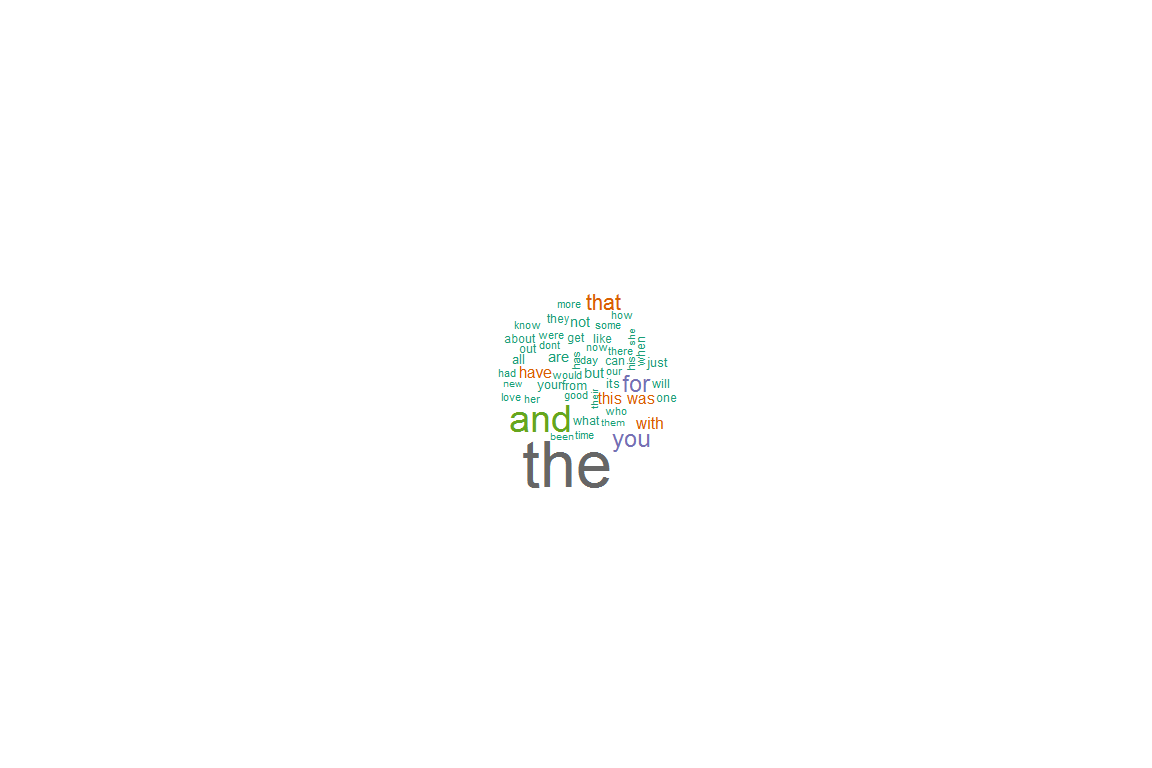
\includegraphics{figure/unnamed-chunk-15-1.pdf}

\paragraph{Random forest prediction}\label{random-forest-prediction}

\begin{Shaded}
\begin{Highlighting}[]
\KeywordTok{set.seed}\NormalTok{(}\DecValTok{12345}\NormalTok{)}
\NormalTok{val_rfmodel <-}\StringTok{ }\KeywordTok{randomForest}\NormalTok{(classe ~}\StringTok{ }\NormalTok{., }\DataTypeTok{data =} \NormalTok{data_pmltraining.train)}
\NormalTok{val_rfmodel.predict <-}\StringTok{ }\KeywordTok{predict}\NormalTok{(val_rfmodel, data_pmltraining.test, }\DataTypeTok{type =} \StringTok{"class"}\NormalTok{)}
\NormalTok{val_rfcm <-}\StringTok{ }\KeywordTok{confusionMatrix}\NormalTok{(val_rfmodel.predict, data_pmltraining.test$classe)}
\NormalTok{val_rfcm}
\end{Highlighting}
\end{Shaded}

\begin{verbatim}
## Confusion Matrix and Statistics
## 
##           Reference
## Prediction    A    B    C    D    E
##          A 2230    0    0    0    0
##          B    2 1518    3    0    0
##          C    0    0 1365    5    0
##          D    0    0    0 1280    0
##          E    0    0    0    1 1442
## 
## Overall Statistics
##                                           
##                Accuracy : 0.9986          
##                  95% CI : (0.9975, 0.9993)
##     No Information Rate : 0.2845          
##     P-Value [Acc > NIR] : < 2.2e-16       
##                                           
##                   Kappa : 0.9982          
##  Mcnemar's Test P-Value : NA              
## 
## Statistics by Class:
## 
##                      Class: A Class: B Class: C Class: D Class: E
## Sensitivity            0.9991   1.0000   0.9978   0.9953   1.0000
## Specificity            1.0000   0.9992   0.9992   1.0000   0.9998
## Pos Pred Value         1.0000   0.9967   0.9964   1.0000   0.9993
## Neg Pred Value         0.9996   1.0000   0.9995   0.9991   1.0000
## Prevalence             0.2845   0.1935   0.1744   0.1639   0.1838
## Detection Rate         0.2842   0.1935   0.1740   0.1631   0.1838
## Detection Prevalence   0.2842   0.1941   0.1746   0.1631   0.1839
## Balanced Accuracy      0.9996   0.9996   0.9985   0.9977   0.9999
\end{verbatim}

Random forest prediction has a reported accuracy against the training
dataset:

\begin{Shaded}
\begin{Highlighting}[]
\KeywordTok{round}\NormalTok{(val_rfcm$overall[}\StringTok{'Accuracy'}\NormalTok{], }\DecValTok{4}\NormalTok{)}
\end{Highlighting}
\end{Shaded}

\begin{verbatim}
## Accuracy 
##   0.9986
\end{verbatim}

\begin{Shaded}
\begin{Highlighting}[]
\KeywordTok{plot}\NormalTok{(val_rfcm$table, }\DataTypeTok{col =} \NormalTok{val_rfcm$byClass, }\DataTypeTok{main =} \KeywordTok{paste}\NormalTok{(}\StringTok{"Random Forest Confusion Matrix: Accuracy ="}\NormalTok{, }\KeywordTok{round}\NormalTok{(val_rfcm$overall[}\StringTok{'Accuracy'}\NormalTok{], }\DecValTok{4}\NormalTok{)))}
\end{Highlighting}
\end{Shaded}

\includegraphics{figure/unnamed-chunk-18-1.pdf}

\paragraph{Generalized boosted regression
prediction}\label{generalized-boosted-regression-prediction}

\begin{Shaded}
\begin{Highlighting}[]
\KeywordTok{set.seed}\NormalTok{(}\DecValTok{12345}\NormalTok{)}
\NormalTok{val_fitControl <-}\StringTok{ }\KeywordTok{trainControl}\NormalTok{(}\DataTypeTok{method =} \StringTok{"repeatedcv"}\NormalTok{, }\DataTypeTok{number =} \DecValTok{5}\NormalTok{, }\DataTypeTok{repeats =} \DecValTok{1}\NormalTok{)}
\NormalTok{val_gbmmodel <-}\StringTok{ }\KeywordTok{train}\NormalTok{(classe ~}\StringTok{ }\NormalTok{., }\DataTypeTok{data =} \NormalTok{data_pmltraining.train, }\DataTypeTok{method =} \StringTok{"gbm"}\NormalTok{, }\DataTypeTok{trControl =} \NormalTok{val_fitControl, }\DataTypeTok{verbose =} \OtherTok{FALSE}\NormalTok{)}
\NormalTok{val_gbmmodel.predict <-}\StringTok{ }\KeywordTok{predict}\NormalTok{(val_gbmmodel, }\DataTypeTok{newdata =} \NormalTok{data_pmltraining.test)}
\NormalTok{val_gbmcm <-}\StringTok{ }\KeywordTok{confusionMatrix}\NormalTok{(val_gbmmodel.predict, data_pmltraining.test$classe)}
\NormalTok{val_gbmcm}
\end{Highlighting}
\end{Shaded}

\begin{verbatim}
## Confusion Matrix and Statistics
## 
##           Reference
## Prediction    A    B    C    D    E
##          A 2232    1    0    0    0
##          B    0 1510    2    0    0
##          C    0    3 1360    3    0
##          D    0    4    6 1282    1
##          E    0    0    0    1 1441
## 
## Overall Statistics
##                                           
##                Accuracy : 0.9973          
##                  95% CI : (0.9959, 0.9983)
##     No Information Rate : 0.2845          
##     P-Value [Acc > NIR] : < 2.2e-16       
##                                           
##                   Kappa : 0.9966          
##  Mcnemar's Test P-Value : NA              
## 
## Statistics by Class:
## 
##                      Class: A Class: B Class: C Class: D Class: E
## Sensitivity            1.0000   0.9947   0.9942   0.9969   0.9993
## Specificity            0.9998   0.9997   0.9991   0.9983   0.9998
## Pos Pred Value         0.9996   0.9987   0.9956   0.9915   0.9993
## Neg Pred Value         1.0000   0.9987   0.9988   0.9994   0.9998
## Prevalence             0.2845   0.1935   0.1744   0.1639   0.1838
## Detection Rate         0.2845   0.1925   0.1733   0.1634   0.1837
## Detection Prevalence   0.2846   0.1927   0.1741   0.1648   0.1838
## Balanced Accuracy      0.9999   0.9972   0.9966   0.9976   0.9996
\end{verbatim}

Generalized boosted regression prediction has a reported accuracy
against the training dataset:

\begin{Shaded}
\begin{Highlighting}[]
\KeywordTok{round}\NormalTok{(val_gbmcm$overall[}\StringTok{'Accuracy'}\NormalTok{], }\DecValTok{4}\NormalTok{)}
\end{Highlighting}
\end{Shaded}

\begin{verbatim}
## Accuracy 
##   0.9973
\end{verbatim}

\begin{Shaded}
\begin{Highlighting}[]
\KeywordTok{plot}\NormalTok{(val_gbmcm$table, }\DataTypeTok{col =} \NormalTok{val_gbmcm$byClass, }\DataTypeTok{main =} \KeywordTok{paste}\NormalTok{(}\StringTok{"Generalized Boosted Regression Confusion Matrix: Accuracy ="}\NormalTok{, }\KeywordTok{round}\NormalTok{(val_gbmcm$overall[}\StringTok{'Accuracy'}\NormalTok{], }\DecValTok{4}\NormalTok{)))}
\end{Highlighting}
\end{Shaded}

\includegraphics{figure/unnamed-chunk-21-1.pdf}

\subsubsection{4. Model Selection}\label{model-selection}

Random forest prediction model is selected due to its superior accuracy.
The expected out-of-sample error is calculated as 1 - accuracy for
predictions made against the cross-validation set:

\begin{Shaded}
\begin{Highlighting}[]
\NormalTok{val_ooserror <-}\StringTok{ }\DecValTok{1} \NormalTok{-}\StringTok{ }\KeywordTok{round}\NormalTok{(val_rfcm$overall[}\StringTok{'Accuracy'}\NormalTok{], }\DecValTok{4}\NormalTok{)}
\NormalTok{val_ooserror}
\end{Highlighting}
\end{Shaded}

\begin{verbatim}
## Accuracy 
##   0.0014
\end{verbatim}

With an accuracy above 99\% on the cross-validation data, it is expected
that few or none of the test samples will be missclassified.

\begin{Shaded}
\begin{Highlighting}[]
\NormalTok{val_rfmodel.final <-}\StringTok{ }\KeywordTok{predict}\NormalTok{(val_rfmodel, data_pmltesting, }\DataTypeTok{type =} \StringTok{"class"}\NormalTok{)}
\NormalTok{val_rfmodel.final}
\end{Highlighting}
\end{Shaded}

\begin{verbatim}
##  2 31  4  5  6  7  8  9 10 11 12 13 14 15 16 17 18 19 20 21 
##  B  A  B  A  A  E  D  B  A  A  B  C  B  A  E  E  A  B  B  B 
## Levels: A B C D E
\end{verbatim}

\subsubsection{5. Coursera Submission}\label{coursera-submission}

\begin{Shaded}
\begin{Highlighting}[]
\NormalTok{pml_write_files =}\StringTok{ }\NormalTok{function(x)\{}
  \NormalTok{n =}\StringTok{ }\KeywordTok{length}\NormalTok{(x)}
  \NormalTok{for(i in }\DecValTok{1}\NormalTok{:n)\{}
    \NormalTok{filename =}\StringTok{ }\KeywordTok{paste0}\NormalTok{(}\StringTok{"problem_id_"}\NormalTok{,i,}\StringTok{".txt"}\NormalTok{)}
    \KeywordTok{write.table}\NormalTok{(x[i], }\DataTypeTok{file =} \NormalTok{filename,}\DataTypeTok{quote =} \OtherTok{FALSE}\NormalTok{, }\DataTypeTok{row.names =} \OtherTok{FALSE}\NormalTok{, }\DataTypeTok{col.names =} \OtherTok{FALSE}\NormalTok{)}
  \NormalTok{\}}
\NormalTok{\}}

\KeywordTok{pml_write_files}\NormalTok{(val_rfmodel.final)}
\end{Highlighting}
\end{Shaded}

\end{document}
